%===================================== KAPITTEL 4 =================================

\chapter{Implementasjon av løsning}
% Dette kapitlet beskriver designet av datamodellevolusjonsløsningen
% Dette kapitlet beskriver også hvordan testingen av datamodellevolusjonsløsningen ble utført

Her følger en skisse av en modulær programvareløsning kalt DBUpgradinator, implementert i Java. De første to delkapitler diskuterer modulens inspirasjoner fra KVolve og problemstillingens måloppnåelseskrav. I det tredje delkapitlet skisseres løsningens tre designmessige perspektiv: Dets fysiske perspektiv; det logiske perspektivet; prosessperspektivet. Dernest skildres kildekoden til modulen. Til sist blir evalueringsprosessen av oppgavens måloppnåelseskrav beskrevet, og et testprogram implementert til inntekt for evalueringen skildres.

\section{Inspirasjoner fra KVolve}

Oppgaven implementerer en frittstående applikasjonsmodul som forsørger støtte for automatisk dataoverføring ved dataaksessering, benevnt som ''lazy data migration'' av \cite{saur2016}, og samtidig tester det ut i et realistisk simulert produksjonsmiljø med datamodellen som vist i \ref{fig1} og \ref{fig2}.

Implementasjonen av migrasjonsløsningen er i stor grad fundamentert på de samme tre sentrale karakteristikkene som KVolve har.

\begin{description}
  \item [Versjonering av aggregat] KVolve kopler sammen logiske versjonsidentifikatorer med aggregatnøkler. Forskjellige versjoner av aggregatene knyttes til forskjellige nøkkelprefiksstrenger, det vil si at at to aggregat som er skrevet innen samme skjemaversjon av applikasjonen har samme nøkkelprefiksstreng. Til eksempel er to aggregat \emph{k:y} og \emph{k:x} begge skrevet under skjemaversjon \emph{k}, derfor identifiseres begge med prefikset \emph{k:}. En applikasjon som sender en spørring til databasen indikerer hvilken skjemaversjon den vil se \citep{saur2016}.
  \item [Oppdaterings-spesifikasjoner og aggregat-transformasjonsfunksjoner] Når en datamodell skal oppgraderes installerer databaseadministratoren en programkompilert spesifikasjon som beskriver det nye versjonsprefikset som identifiserer versjonen til det neste dataskjemaet, samt en mengde aggregat-transformasjonsfunksjoner som brukes til å oppgradere visse aggregater. Enhver transformasjonsfunksjon har et prefiks i sitt navn, \emph{p} som indikerer skjemaversjonen til aggregater funksjonen skal kalles på.
  \item [Aggregat-transformasjon ved dataaksess] Aggregater lagret i KVolve blir ikke automatisk oppgradert når en ny oppdateringsspesifikasjon installeres i databasen. Når en ny versjon av applikasjonstjeneren starter vil den handtere brukerforespørsler og deretter sende GET og SET - operasjoner til databasen. Hvis en GET - operasjone treffer et aggregat som har en eldre skjemaversjon men ikke den nyeste, vil en transformasjonsfunksjon kalles for å oppgradere aggregatet slik at det kan returneres til applikasjonsinstansen med den nyeste skjemaversjonen. Hvert enkelt aggregat blir altså oppgradert ved forespørsel, og ikke på ivrig, tvungen vis som direkte respons på at en oppgradering er kommisjonert. I KVolve blir applikasjonsinstanser hvis skjemaversjon er utdatert automatisk frakoplet databasen og får ikke lov til å sende forespørsler. Således hindrer \cite{saur2016} et mikset versjonsmiljø og sikrer konsistente skjemaversjoner.
\end{description}

Oppgavens programvareløsning, DBUpgradinator, er preget av noen annerledes designvalg som passer bedre til en likemannsarkitektur. Det mest vesentlige avviket er at datamodelloppgraderingen tillater miksing av skjemaversjoner blant applikasjonstjenerne. Om datamodellen må oppgraderes på grunn av endringer i applikasjonslogikken så skal ikke det gå utover tjenesteytelsen til de uoppgraderte applikasjonstjenerne her og nå. For DBUpgradinator kan vi ha persistert to aggregat, \emph{k:x} og \emph{j:x}, som begge i prinsippet peker på samme ''dataobjekt'', men for to forskjellige skjemaversjoner. Dette scenariet er ikke tillatt i KVolve.

Et annet designmessig avvik ligger i programmeringsspråket brukt til å implementere DBUpgradinator, Java. Proof-of-concept - implementasjonen av KVolve er skrevet i C. I et objektorientert språk som Java kan klasser brukes til å modellere oppdateringsspesifikasjonen. En klasse kalt `AbstractAggregateTransformer` realiserer både oppdateringsspesifikasjonen, ved å holde på to tilstandsvariable som indikerer navnet på en skjemaversjon som kommer før en annen, og dets transformasjonsfunksjon.

KVolve - implementasjonen til \cite{saur2016} kan også brukes til å oppgradere applikasjonstjenere, i artikkelen brukes Redis - modulen \underline{Amico} som et praktisk eksempel.

\section{Krav til implementasjon av levende datamigrasjonsløsning}

Her følger de funksjonelle og ikke-funksjonelle krav som stilles til programvaremodulen som skal kunne migrere data fra et implisitt aggregatskjema til det neste uten stans i dataleveranser på brukernes tjenesteforespørsler.

\subsection{Antakelser}

I kraft av å demonstrere et praktisk konsept vil modulen gjøre visse antakelser om programvarearkitekturen til den jevne webapplikasjon DBUpgradinator kommer til å operere i. Enkelte av disse fordringene er gjort for å gjøre den objekt-orienterte implementasjonen av datamodellevolusjonsløsningen mindre parametrisert og derfor enklere og skrive og enklere å forstå.

For å realisere tillatelsen av versjonsmiks mellom forskjellige applikasjonstjenere i webapplikasjonen DBUpgradinator er installert i vil dets implementasjon ikke oppdatere aggregater direkte, men heller lage et nytt et med et annerledes streng-prefiks. Følgelig vil den samme ''tuppelen'' lagres dobbelt opp hvis miksen av skjemaversjoner er av størrelse 2.

Her listes øvrige antakelser for prototypeimplementasjonen av DBUpgradinator, databasen den kommer til å operere på, webapplikasjonen den testes i, og produksjonsmiljøet DBUpgradinator testes i.

\begin{itemize}
  \item Dataobjekter serialiseres 'client' side, altså er lagringsnodene 'dumme' og backend-tjenerne 'smarte'
  \item Serialisering (Voldemort): \underline{String}, altså ser den enkelte databasetjener kun strenger og kan ikke lese av skjemaet; videre antas det at databasen bruker LWW - strategien for å løse flettetvister automatisk
  \item Applikasjonsstakken til Voldemort-instansen denne oppgaven tester har en fast konfigurasjon
  \item Nøkler i skjemaet endrer ikke type eller form
  \item Dataobjekter har en skjema-versjonstag brukt til å sjekke om tuppelen må oppgraderes
  \item Fordi modulen i prinsippet må være skjemaopplyst må den implementeres som en del av applikasjonslogikken
  \item Oppdateringsspesifikasjoner kan kjedes sammen, denne kjeden har Migrator-klassen styr på, altså er det Migrator-klassen som har en tilstandvariabel som peker på en lenket liste av instanser av transformasjonsobjekter
  \item Akkurat som med KVolve blir ikke disse transformeringsobjektene fjernet når alle aggregatene lagret på det gamle skjemaet er migrert ferdig
  \item Applikasjonen, skrevet i Java, holder styr på sitt implisitte skjema gjennom eksplisitt versjonering og eksplisitt deklarering av aggregatets modell ved å definere en egen Aggregate-klasse
  \item Webapplikasjonens utviklere programmerer på et eget lokalt utviklingsmiljø
  \item I serversiden er tupler lagret med nøkler på form k:x, der suffikset x indikerer skjemaversjonen. Disse dataobjektene har ingen separate versjonsfelt idet de sendes Voldemort-serveren
  \item Den enkelte utvikler har ikke behov for å endre nøkkelens struktur eller datatype
  \item Alle nøkler Voldemort mottar er på strengform, selv om nøkler i praksis også kan være en liste av binærdata, derfor støtter ikke DBUpgradinator nedring av nøkkelens skjemastruktur
  \item Webapplikasjonen som modulen testes i har en RESTful - arkitektur
  \item For ett bestemt produksjonsmiljø er det til enhver tid kun én klientinstans som kommuniserer med de andre; denne klientinstansen sender til enhver tid transformasjonsobjekter i ordentlig rekkefølge, det vil si at klienten gjør seg ferdig med å sende ett transformasjonsobjekt for én skjemaversjon til alle applikajsonstjenere før denne sender over transformasjonsobjektet som gjelder for den etterfølgende versjonen
  \item Når transformasjonsobjekter sendes, så sendes de i en bestemt rekkefølge, altså er ikke rekkefølgen applikasjonstjenere mottar transformatorer i tilfeldig - denne antakelsen tillater oss å spesialisere og forenkle enkelte detaljer av kildekoden som kjører hos applikasjonsinstansene
  \item Til enhver tid oppgraderes applikasjonen kun én versjon ad gangen, det vil si at på det meste er to forskjellige utgaver av versjonen som opererer i produksjonsmiljøet på ett og samme tidspunkt
\end{itemize}

\subsection{Funksjonelle krav}

\begin{enumerate}
  \item DBUpgradinator er en modul som skal kjøre i produksjonsmiljøet til en webapplikasjon skrevet i Java
  \item DBUpgradinator skal lage én ekstra databasespørring for hver nye transformasjon som påføres et aggregat
  \item Ved en GET-forespørsel til aggregatet med nøkkel \emph{x} fra en applikasjonsinstans som bruker en ny skjemaversjon \emph{k} skal DBUpgradinator også opprette en GET-forespørsel etter det samme aggregatet men med prefikset til den foregående skjemaversjonen i nøkkelen, \emph{j}
  \item Hver enkelt applikasjonsinstans har kontroll over versjonen av dataskjemaet sitt, som identifiseres ved en hashstreng som konkatineres med IDen til hver enkelt dataelement før PUT sendes til databasen
  \item Oppgraderingsverktøyet vil opprette en ny tuppel i lageret hvis skjema-versjon-suffiks er annerledes og dataobjekt-ID-prefiks er likens prefikset til tuppelen som oppgraderes; således kan det distribuerte systemet kjøre en mikset tilstand mens datamigrasjonen foregår
  \item Ved kjøring av DBUpgradinator: Hvis programmet mottar en spørring etter et aggregat som tilhører den nyeste skjema-versjonen (f.eks en GET på en nøkkel hvis skjemaversjon-suffiks tilsvarer versjonsstrengen til den nyeste skjemaversjonen) så vil ikke en migrasjon med transformator-klassen bli utført
\end{enumerate}

\subsection{Kvalitetskrav}

\begin{enumerate}
  \item Tilgjengelighet: Det skal være mulig å forespørre data fra databasen mens datamigrasjon er iverksatt. Dette kravet evalueres ikke på kvantitativt, men på kvalitativt grunnlag, det vil si ved å kjøre DBUpgradinator i et simulert produksjonsmiljø, det vil si en applikasjon som ikke mottar forespørsler fra klienter som kommuniserer med HTTP.
  \item Ytelse: Ved rullerende eller lat datamigrasjon utsettes databasen for en vesentlig degradering i gjennomstrømskapasitet, målt i spørringer per sekund. Denne hemmelsen må være minimal i den implementerte migrasjonsløsningen.
  \item Modularitet: Løsningen som programmeres bør interferere minst mulig med eksisterende kildekode i Project Voldemort, primært gjennom å utvikle det som et separat prosjekt.
\end{enumerate}

\section{Modeller}

Her følger uformell dokumentasjon over dataevolusjonsmoculen DBUpgradinator og hvordan den skal oppføre seg i en datadreven webapplikasjon hvis dataelementer persisteres i en distribuert database. Dokumentasjonen er basert på 4+1-metamodellen Phillippe Kruchten presenterer i en artikkel fra 1995.

\subsection{4+1 - stilen}

Dokumentasjon av programvarearkitektur er en kommunikasjonskunst. Symbolene som tegnes på et lerret eller på en bildefil bærer ingen betydning eller mening i seg selv, hva de representerer er noe dokumentets forfattere og dets påtenkte publikum må være samstemte om. Videre er tydelige kommuniserende begrenset når det kommer til hvor mange konsepter de kan representere på ett og samme tidspunkt. En firkant, eller en boks, kan til eksempel ikke representere både en statisk fil med programkode i og samtidig en kjørende prosess. Enkelte arkitekturdokumenter fokuserer for mye på ett enkelt aspekt ved datasystemet, eller tar ikke hensyn til ønsker og bekymringer til samtlige interessenter, de distinkte gruppene som leser dokumentet. Derfor foreslår \cite{kruchten1995} å organisere dokumentasjonen til en programvarearkitektur inn i en mengde av fire perspektiv (eng. viers) som hver for seg besvarer ett spesifikk interesseområde for applikasjonen.

Disse fire perspektivene kaller \cite{kruchten1995} for:
\begin{description}
  \item [Det logiske perspektivet] I kontekst av objekt-orientert programmering er dette en oversikt over objekter (teknisk sett prosesser/tråder) som eksisterer i primærminnet til datamaskinene i systemet
  \item [Prosessperspektivet] Gir leseren en oversikt over detaljer angående samtidige operasjoner og synkronisering i systemets design
  \item [Det fysiske perspektivet] Beskriver 1) koplingene mellom programvareelementer og maskinvareelementer i systemet og 2) systemets distribuerte naturBeskriver 1) koplingene mellom programvareelementer og maskinvareelementer i systemet og 2) systemets distribuerte natur
  \item [Utviklingsperspektivet] Beskriver programvarens statiske organisering av dets kildekode i utviklermiljøet
\end{description}

Den primære oppgaven til det logiske perspektivet av arkitekturdokumentasjonen er å representere effektene de funksjonelle krav som stilles til datasystemet har på det. De funksjonelle krav har opprinnelse i domenet til problemet datasystemet angriper. Systemets viktigste abstrakte konstruksjoner, kalt objekter i programmets og klasser i kildekoden, kan knyttes til separate begreper inneholdt i domenet til problemet interessentene (de som leser arkitekturdokumentet) vil løse \citep{kruchten1995}. Objekter utnytter egenskaper som arv/spesialisering, innkapsling og funksjonsmaskering gjennom grensesnitt for å realisere påkrevd funksjonalitet. Logiske perspektiver inneholder gjerne klassediagrammer og sekvensdiagrammer skrevet med UML - syntaksen. Et klassediagram viser en oversikt over klassene og relasjoner mellom dem i et objekt-orientert program. Hvis applikasjonen er sterkt datadrevet, slik tilfelle gjerne er i kommersielle webapplikasjoner som netthandel-informasjonssystemer, er det hensiktsmessig å presentere et ER -  eller et EER - diagram i det logiske perspektivet også.

Prosessperspektivet beskriver hvordan oppfører seg når det kjører og hvordan det kjører. Prosessperspektivet reflekterer de ikke-funksjonelle krav, herunder kvalitetskrav, oppførselskrav og begrensende krav, som stilles til datasystemet. Sentrale problemer som tas stilling til inkluderer samtidighet, feiltoleranse, distribusjon av arbeidslast, integritet, parallelt kjørende tråder og hvordan entiteter, klasser eller objekter fra det logiske perspektivet gjenspeiles i prosessperspektivet \citep{kruchten1995}. Her svarer et objekt fra det logiske perspektivet til en tråd underordnet en kjørende prosess i et operativsystem. Et høytilgjengelig system vil typisk modelleres slik at enhver slik prosess i systemet har en identisk tvilling som kan steppe inn og ta over sin partners arbeidslast skulle den svikte, også kjent som en reserveprosess, på engelsk kalt for ‘’spare’’.

Oppgaven til programvarearkitekturdokumentasjonens fysiske perspektiv er å definere sammenhengen mellom kildekode og maskinvaren (m.a.o. datamaskiner) som koden kjører på. Perspektivet er særskilt relevant for systemer der strenge, spesifikke krav stilles dets ytelse (gjennomstrømming i fore eksempel antall transaksjoner per sekund), tilgjengelighet (evnen til å handtere delvis eller fullstendig svikt) og pålitelighet (feiltoleranse). Arkitekturen til et distribuert system består av et nettverk av uavhengige datamaskiner som prosesserer data, kalt \emph{noder}. Derfor er det vesentlig å dokumentere hvilken rolle de abstrakte programvareelementer fra prosessperspektivet og utviklingsperspektivet spiller i forhold til de forskjellige fysiske noder \citep{kruchten1995}. Systemet har vanligvis forskjellige konfigurasjoner, en mengde parametere som bestemmer programvarens oppførsel under kjøretid. Én konfigurasjon kan gjelde for systemets testfase, en annen for når dets produksjonsmiljø, og et atter annet for vedlikeholds- eller utviklingsmiljø \citep{kruchten1995}. De forskjellige konfigurasjoner illustreres ofte i hvert sitt distribusjonsdiagram, som også kan skisseres med UML-syntaks.

Utviklingsperspektivet tiltaler primært applikasjonens utviklere og vedlikeholdere, de som skal endre dets kildekode. Programmet inndeles i mindre enheter, kalt ‘’bibliotek’’ eller ‘’moduler’’, hvilket kan refereres til og benyttes av utviklere på tvers av store eller små prosjektgrupper. Disse modulene er organisert hierarkisk i forskjellige \emph{lag}, det vil si at hver modul eksponerer et veldefinert programmeringsgrensesnitt som andre moduler organisert direkte ‘’oppå’’ den kan kalle på uten å være involvert i bibliotekets kildekode. Diagrammer innen utviklingsperspektivet viser derfor typisk import/eksport - forhold imellom forskjellige programvaremoduler, som i tur også kan samles sammen inn i pakker, som best kan beskrives som ‘’meta-moduler’’. Selv om utviklingsperspektivet ikke er komplett før samtlige programvareelementer i systemet er definert og navngitt kan det deklarere de regler som bestemmer kildekodeorganiseringens natur, deriblant eksponering av funksjoner via import/eksport av bibliotek, gruppering av moduler inn i pakker, og avgrensning av moduler. Utviklingsperspektivet er nyttig primært for ansvarsfordeling og å gjøre konkrete implementasjonsvalg som valg av språk, utviklingsverktøy og tredjepartsmoduler lettere.

Disse fire separate perspektivene kan også kombineres sammen i et femte perspektiv, kalt bruksscenarier, som oppsummerer systemets mengde av funksjonelle krav \citep{kruchten1995}. Meningen bak dekomponeringen av programvarearkitekturdokumentasjonen er å belyse vesentlige interesseområder av systemet. Det er vesentlig å notere at perspektivmodellen i all hovedsak er en metamodell - en beskrivelse av sammenhengen mellom konkrete modeller for programmet brukt i arkitekturens dokumentasjon. Videre må det nevnes at samtlige perspektiver i metamodellen er valgfrie, enhver arkitekt står fri til å gjøre justeringer på sitt dokument i henhold til de krav som stilles systemarkitekturen som modelleres. DBUpgradinator modelleres med de tre første perspektivene i 4+1-metamodellen. Ettersom prosjekter er et enmannsarbeid er et sett av diagrammer som utgjør et eget utviklingsperspektiv ikke strengt nødvendig. Ett perspektiv som i kontekst av distribuerte applikasjoner er uunnværlig er det fysiske perspektivet.

\subsection{Det logiske perspektiv}

Klassene som refereres til i diagrammene:
\begin{itemize}
  \item \textbf{AbstractAggregateTransformer} - en abstrakt klasse med en tilstandsvariabel som indikerer applikasjonsversjonen oppgraderingsklassen opererer på og en som indikerer nøkkelverdien til den neste applikasjonen som den transformerte verdien gjelder for; klassen har én abstrakt metoder, som implementeres i subklassen programmert og kompilert til \texttt{.class}-fil av den individuelle applikasjonsprogrammerer. Metodens navn er \texttt{TransformAggregate}, som påkalles når en forespørsel fra webapplikasjonens gamle versjon (som er under rullerende oppgradering) tilsendes databaseklienten, den påkalles både når klienten mottar data fra datalageret, etter at en \texttt{InconsistencyResolver} har flettet divergerende elementer; argumenter: key (fra DB), value (deserialisert), så vel som når klienten mottar data fra applikasjonen, altså fra forespørselen direkte.
  \item \textbf{AppVersionResolver} - hjelperklasse som kopler dataobjektets nøkkel i en innkommende HTTP-spørring (k) med applikasjonsversjonens nøkkel (x) på formen \texttt{k + ":" + x}
  \item \textbf{AggregateTransformerReceiver} - frittstående prosess som ikke er del av en spørrings livsløp, men som både mottar AggregateTransformer-objekter og holder rede på dem i versjonsrekkefølge i en privat liste. Har også ansvar for å påkalle transformasjonsmetoden til hvert objekt.
  \item \textbf{Migrator} - \texttt{public} hovedklasse som eksponerer DBUpgradinator sin funksjonalitet til programvareutvikleren. Dens tilstand inkorpurerer aggregatets objekttype - det vil si domeneklassen til aggregatet, som sendes inn i transformasjonsfunksjonen til AbstractAggregateTransformer-klassen som verdi-argument. Transformasjonsfunksjonen blir overridet av den implementerte klassen.
\end{itemize}

\newpage

% Figur 5
\begin{figure}[!ht]
    \centering
    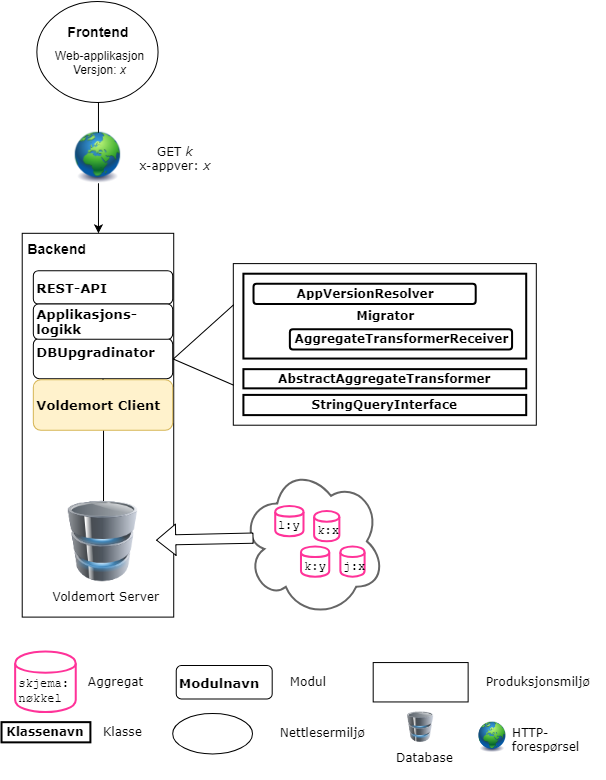
\includegraphics[scale=0.5]{fig/dbupgradinator-logisk-1.png}
    \caption{Logisk oversikt over moduler i det typiske produksjonsmiljøet DBUpgradinator opererer i. Klassene som DBUpgradinator består av nevnes med navn.}
    \label{fig5}
\end{figure}

\newpage

% Figur 6
\begin{figure}[!ht]
    \centering
    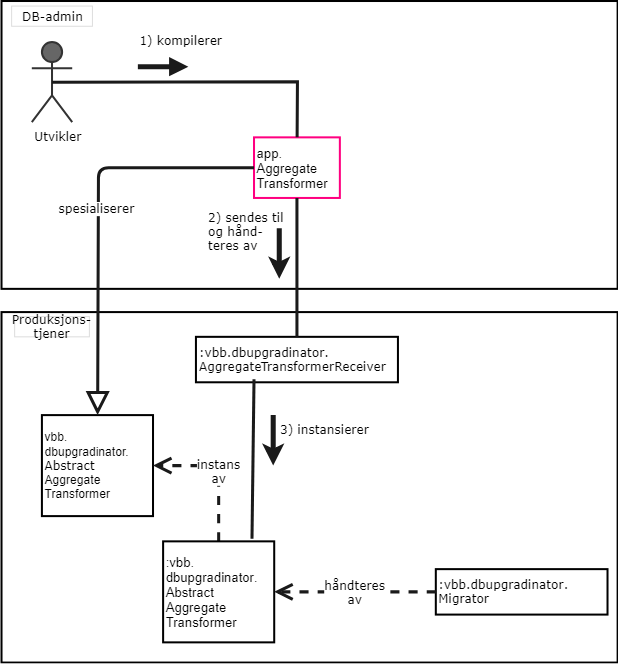
\includegraphics[scale=0.5]{fig/dbupgradinator-logisk-2.png}
    \caption{Logisk oversikt over moduler i det typiske produksjonsmiljøet DBUpgradinator opererer i. Klassene som DBUpgradinator består av nevnes med navn.}
    \label{fig6}
\end{figure}

\newpage

\subsection{Det prosessmessige perspektiv}

% Figur 7
\begin{figure}[!ht]
    \centering
    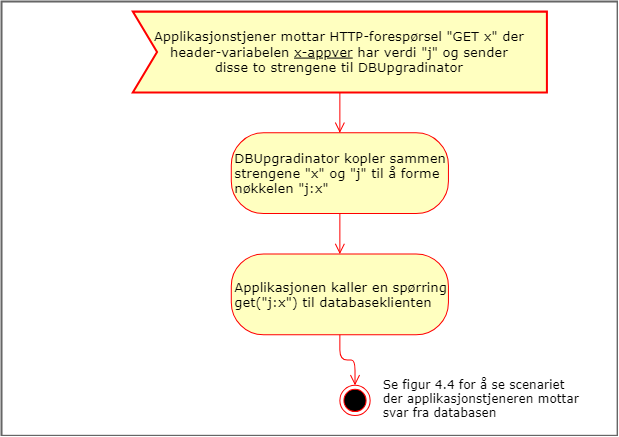
\includegraphics[scale=0.6]{fig/dbupgradinator-prosess-1.png}
    \caption{Prosess.}
    \label{fig7}
\end{figure}

\newpage

% Figur 8
\begin{figure}[!ht]
    \centering
    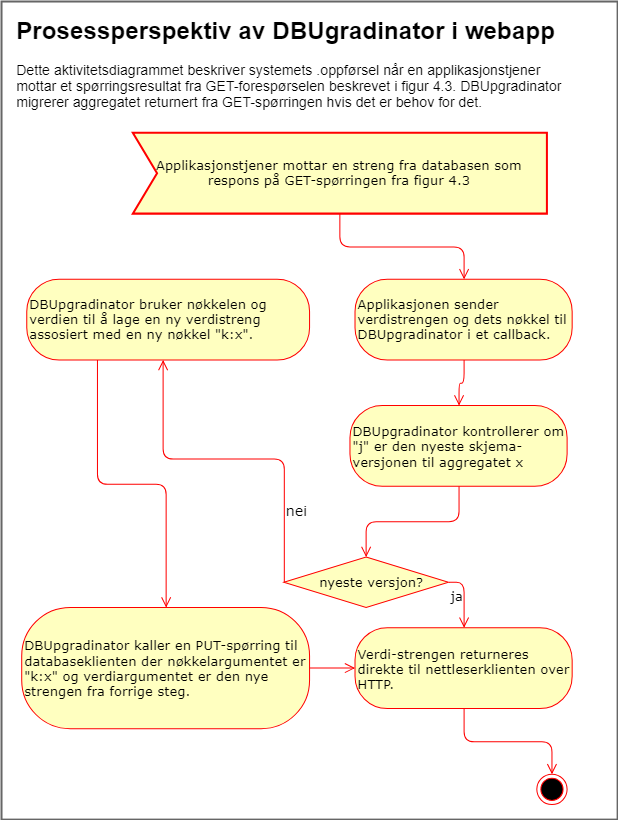
\includegraphics[scale=0.6]{fig/dbupgradinator-prosess-2.png}
    \caption{Prosess.}
    \label{fig8}
\end{figure}

\newpage

% Figur 9
\begin{figure}[!ht]
    \centering
    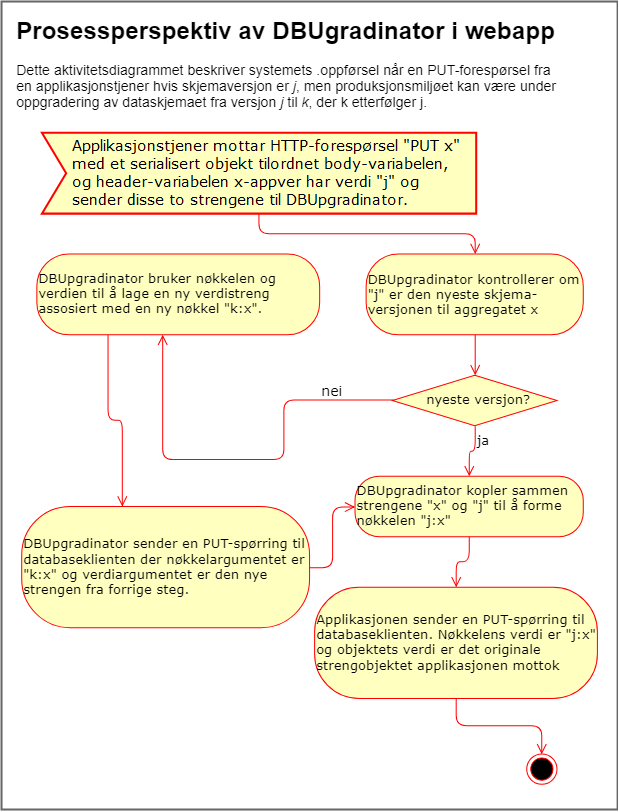
\includegraphics[scale=0.6]{fig/dbupgradinator-prosess-3.png}
    \caption{Prosess.}
    \label{fig9}
\end{figure}

\newpage

\subsection{Det fysiske perspektiv}

% Figur 10
\begin{figure}[!ht]
    \centering
    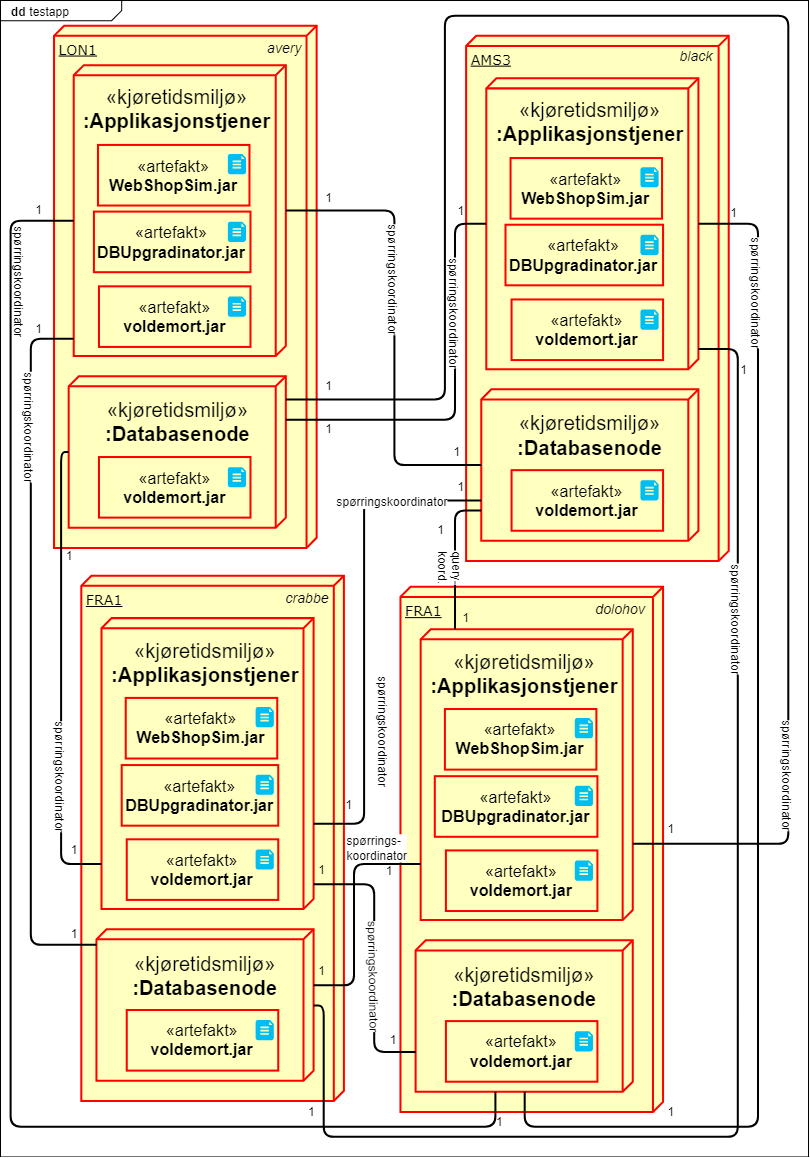
\includegraphics[scale=0.6]{fig/dbupgradinator-physical.png}
    \caption{Deployment-diagram.}
    \label{fig10}
\end{figure}


\cleardoublepage
